\documentclass[a4paper,12pt]{article}
\usepackage[swedish]{babel}
\usepackage[utf8]{inputenc}
\usepackage{amsmath, amsthm, amssymb}
\usepackage{graphicx}
\usepackage{enumitem}
\usepackage[a4paper,includeheadfoot,margin=2.54cm]{geometry}
\begin{document}
%
\section{Dugga 5 - Fråga 8}
Hur många ord kan bildas av VINGUMMIN där varken II, NN eller MM förekommer?
\subsection*{Svar}
Vi börjar med att räkna det totala antalet av ord som går att bilda. Vi har
\begin{align}
  1 \text{ V, } 2 \text{ I, } 2 \text{ N, } 1 \text{ G, } 1 \text{ U, } 2 \text{ M}.
\end{align}
och det är totalt 9 bokstäver. Alltså blir det
\begin{align}\label{eq1}
    \frac{9!}{1! \cdot 2! \cdot 2! \cdot 1! \cdot 1! \cdot 2!} = 45367
\end{align}
och för att se till att inga dubletter förekommer börjar vi med att räkna de
arrangemang där mins en dublett förekommer och räknar det som en enhet
\begin{align}
    \frac{8!}{1! \cdot 1! \cdot 2! \cdot 1! \cdot 1! \cdot 2!} = 10080
\end{align}
och eftersom det finns $\binom{3}{1} = 3$ sätt att välja vilket par som
förekommer, så multiplicerar vi svaret med $3$.
\begin{align}\label{eq2}
    10080 \cdot 3 = 30240.
\end{align}
Nu räknar vi antalet arrangemang där 2 dubletter förekommer
\begin{align}
    \frac{7!}{1! \cdot 1! \cdot 1! \cdot 1! \cdot 2!} = 2520
\end{align}
och eftersom det finns $\binom{3}{2} = 3$ sätt att välja vilka två par som
förekommer multiplicerar vi med 3 här också
här med
\begin{align}\label{eq3}
    2520 \cdot 3 = 7560.
\end{align}
Sedan räknar vi på när alla 3 par förekommer
\begin{align}\label{eq4}
    \frac{6!}{1! \cdot 1! \cdot 1! \cdot 1! \cdot 1! \cdot 1!} = 6! = 720
\end{align}
nu måste vi ta hänsyn till dubbelräkning, och det gör vi genom att ta uträkning
\ref*{eq2} subtraherat med uträkning \ref*{eq3} och sist adderat med uträkning
\ref*{eq4}
\begin{align}
    30240 - 7560 + 720 = 23400
\end{align}
och till sist för att få veta hur många ord som kan bildas av VINGUMMIN där
inga dubletter förekommer tar vi totala antalet ord subtraherat med de oönskade
fallen
\begin{align}
    45367 - 23400 = 21960.
\end{align}
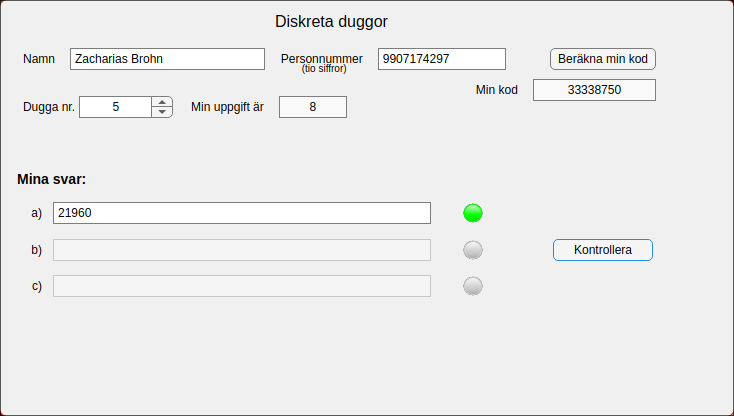
\includegraphics[width=\textwidth]{RMXBJIG.png}
%
\end{document}
%
\end{document}
